% TCSE 2026 — 中文一般論文（目標 5 頁）
% 編譯器：pdfLaTeX（Overleaf 預設，不需更改任何設定）
\documentclass[conference]{IEEEtran}
\IEEEoverridecommandlockouts

\usepackage{CJKutf8}
\usepackage{amsmath,amssymb,amsfonts}
\usepackage{graphicx}
\usepackage{booktabs}
\usepackage{multirow}
\usepackage{xcolor}
\usepackage{cite}
\usepackage{url}
\usepackage{hyperref}
\hypersetup{colorlinks=true,linkcolor=blue,citecolor=blue,urlcolor=blue}

\begin{document}
\begin{CJK}{UTF8}{bkai}

\title{面向工業設備健康監測之可重現無監督異常偵測軟體流程：\\
以 VAE 軸承振動分析為例}

\author{
\IEEEauthorblockN{作者姓名}
\IEEEauthorblockA{
\textit{系所名稱}\\
\textit{學校名稱}\\
台灣\\
email@xxx.edu.tw}
}

\maketitle

% ─────────────────────────────────────────────────────
\begin{abstract}
工業設備健康監測長期面臨兩大挑戰：故障資料稀少且標注成本高昂，
以及現有研究因資料切分不當而產生難以重現的過樂觀結果。
本研究設計並開源一套\textbf{可重現的無監督異常偵測軟體流程}，
以變分自編碼器（VAE）為核心演算法，
從資料自動下載、工廠情境平衡、模型訓練至結果視覺化全程自動化，
並明確記錄各階段設計決策以確保實驗可重現性。
流程僅使用正常振動訊號進行訓練，透過 KL 散度將潛在空間正則化至標準常態分布，
形成「正常潛在流形」，故障訊號因落在流形之外而產生高重建誤差，藉此實現偵測。
以凱斯西儲大學（CWRU）軸承振動資料集為案例，
模擬工廠真實不平衡分布（正常 79.5\%：故障 20.5\%），
五折交叉驗證達到 AUC-ROC $= \mathbf{1.0000 \pm 0.0000}$，
故障重建誤差為正常訊號之 5.2 倍。
消融實驗驗證流程在不同超參數下均具穩健性。
本研究之完整程式碼與實驗結果已公開於 GitHub，
供工業 AI 研究者重現與延伸應用。
\end{abstract}

\begin{IEEEkeywords}
無監督異常偵測，變分自編碼器，可重現軟體流程，工業健康監測，軸承故障，開源工具
\end{IEEEkeywords}

% ─────────────────────────────────────────────────────
\section{研究背景與動機}
% ─────────────────────────────────────────────────────

旋轉機械設備中，軸承故障約佔馬達失效原因的 40--50\%\cite{smith2015rolling}，
一旦發生非計畫性停機，不僅造成高額維修成本，更可能引發安全事故。
根據工業統計，非計畫性停機每小時損失可高達數萬至數十萬美元，
因此建立能在故障發生前即時預警的可信賴偵測系統，是智慧製造領域的核心課題之一。

傳統監督式學習方法（如支援向量機 SVM、卷積神經網路 CNN）
在實際部署時面臨兩大根本性挑戰：
（一）\textbf{資料不平衡}：工廠正常運作期間故障事件極為罕見，
故障樣本數量遠少於正常樣本，導致分類器偏向多數類別；
（二）\textbf{標注成本高昂}：蒐集並標注故障資料需要領域專家介入，
且往往需要刻意引發設備損壞以取得各類故障樣本，難以在生產環境中規模化執行。

生成模型提供了突破上述瓶頸的解法：只需學習正常資料的分布，
於推論時將偏離此分布的樣本視為異常，無需任何故障標注。
其中，變分自編碼器（Variational Autoencoder, VAE）\cite{kingma2014auto}
因具備：（a）明確的機率性潛在空間、（b）幾何上可解釋的正則化結構、
（c）端對端訓練的工程易用性，成為工業異常偵測的優選架構。

本研究的四項主要貢獻如下：
\begin{enumerate}
  \item \textbf{可重現開源軟體流程：}提出一套模組化、全自動的異常偵測管線，
        從 CWRU 資料集自動下載、視窗切割、工廠情境平衡、VAE 訓練至結果視覺化，
        完整程式碼公開於 GitHub，所有實驗結果可一鍵重現。
  \item \textbf{工廠真實情境模擬：}明確設計資料不平衡策略，
        保留全部 3,310 筆正常資料，隨機保留 10\% 故障資料（852 筆），
        比率 79.5:20.5，比多數文獻使用平衡資料集更貼近真實部署場景。
  \item \textbf{無標籤訓練策略：}VAE 訓練期間完全不接觸故障資料，
        所學習的正常潛在流形可直接應用於未見過的故障類型，
        不受故障標注成本限制。
  \item \textbf{系統性消融驗證：}以五折交叉驗證與多組消融實驗（KL 權重、潛在維度）
        全面記錄各設計決策的效果，提供後續研究者明確的超參數選擇依據。
\end{enumerate}

% ─────────────────────────────────────────────────────
\section{相關研究}
% ─────────────────────────────────────────────────────

\subsection{傳統訊號特徵方法}
早期研究以時頻域統計特徵（均方根值、峰度、峰值因數、頻率重心等）
搭配支援向量機或 $k$ 近鄰分類器進行故障辨識\cite{smith2015rolling}。
快速傅立葉轉換（FFT）與短時傅立葉轉換（STFT）可揭示特征故障頻率，
但解讀需要大量領域專業知識，且模型效能高度依賴特徵設計品質與充足的標注資料，
限制了在實際工業場景中的推廣應用。

\subsection{深度學習監督式方法}
卷積神經網路（CNN）與長短期記憶網路（LSTM）直接對原始訊號或頻譜圖進行分類，
在 CWRU 等標準資料集上已達到 99\% 以上之準確率\cite{zhao2019deep}。
然而此類方法仍需大量標注的故障資料，在資料不平衡或標注稀缺的真實場景中
效能明顯退化，且對於訓練期間未見過的故障模式泛化能力有限。

\subsection{無監督異常偵測}
自編碼器（AE）透過重建誤差進行異常評分，僅需正常資料即可訓練\cite{an2015variational}。
VAE 在 AE 基礎上引入 KL 散度正則化，明確約束潛在空間分布，
使正常資料的潛在表徵形成緊湊的幾何流形，提升異常樣本的可辨識性。
近年亦有研究探討生成對抗網路（GAN）與流模型（Normalizing Flow）於異常偵測的應用，
但訓練穩定性較低且架構複雜，不利於工業部署。
本研究在 VAE 基礎上，進一步針對一維振動訊號最佳化卷積架構，
並以系統性消融實驗驗證設計選擇。

% ─────────────────────────────────────────────────────
\section{系統設計}
% ─────────────────────────────────────────────────────

\subsection{資料集與前處理}

本研究使用凱斯西儲大學軸承振動資料集\cite{loparo2012}，
包含 SKF 6205 深溝球軸承在 12,000 Hz 取樣頻率下，
三種故障類型（內圈、滾動體、外圈）、三種損傷尺寸（0.007"、0.014"、0.021"）
與四種負載條件（0--3 HP，對應 1,720--1,797 RPM）的振動訊號，共 40 個 .mat 檔案。

\textbf{滑動視窗切割：}以 1,024 點（$\approx$85 ms at 12 kHz）為視窗，
512 點為步長（50\% 重疊），切割出 11,832 片段（正常 3,310 筆，故障 8,522 筆）。
圖~\ref{fig:timedomain} 展示四類訊號之時域波形，
可見故障訊號具有明顯週期性衝擊特徵。

\begin{figure}[ht]
  \centering
  \includegraphics[width=0.95\columnwidth]{time_domain.png}
  \caption{四類軸承訊號之時域波形比較。正常訊號（藍）呈現穩定隨機振動；
  三類故障訊號均出現週期性衝擊，內圈（紅）、滾動體（橙）、外圈（紫）
  各具不同的衝擊頻率特徵。}
  \label{fig:timedomain}
\end{figure}

\textbf{工廠情境平衡：}保留全部 3,310 筆正常片段，
隨機保留 10\% 故障片段（共 852 筆，其中內圈 282、滾動體 271、外圈 299），
總計 4,162 筆（正常佔 79.5\%），模擬真實工廠的資料不平衡分布。

\textbf{標準化：}對每個視窗獨立進行 Z-score 標準化（零均值、單位標準差），
消除不同負載條件下的振幅偏差。

\subsection{VAE 架構設計}

\textbf{編碼器：}四層步幅卷積將輸入 $(B,1,1024)$ 逐步壓縮，
$\text{Conv}(1\to16, k=7, s=2)$、$\text{Conv}(16\to32, k=5, s=2)$、
$\text{Conv}(32\to64, k=3, s=2)$、$\text{Conv}(64\to128, k=3, s=2)$，
各層搭配批次正規化（Batch Normalization）與 ReLU 激活。
展平後經全連接層 $\text{FC}(8192\to256\to32)$ 分別輸出均值 $\boldsymbol{\mu}$
與對數變異數 $\log\boldsymbol{\sigma}^2$（各 32 維）。

\textbf{重參數化技巧：}
\begin{equation}
  \mathbf{z} = \boldsymbol{\mu} + \boldsymbol{\varepsilon} \odot
  \exp\!\left(\tfrac{1}{2}\log\boldsymbol{\sigma}^2\right),\quad
  \boldsymbol{\varepsilon} \sim \mathcal{N}(\mathbf{0},\mathbf{I})
\end{equation}
此技巧允許梯度透過隨機採樣步驟回傳，使整體架構可端對端訓練。

\textbf{解碼器：}全連接層 $\text{FC}(32\to256\to8192)$ 擴展潛在向量，
整形後經四層轉置卷積（ConvTranspose1d）重建長度 1,024 的訊號，
最終以 Tanh 激活限制輸出範圍。

\subsection{損失函數}

\begin{equation}
  \mathcal{L} =
  \underbrace{\mathrm{MSE}(x,\hat{x})\times 1024}_{\text{重建損失 (Reconstruction)}}
  +\;\beta\cdot
  \underbrace{D_{\mathrm{KL}}\!\left(q(\mathbf{z}|x)
  \,\|\,\mathcal{N}(\mathbf{0},\mathbf{I})\right)}_{\text{KL 散度 (Regularisation)}}
\end{equation}

KL 散度的解析式為：
\begin{equation}
  D_{\mathrm{KL}} = -\frac{1}{2}\,\mathrm{mean}\!\left(
  1 + \log\sigma^2 - \mu^2 - e^{\log\sigma^2}\right)
\end{equation}

本研究使用 $\beta=1.0$（標準 VAE）。KL 項迫使正常資料的潛在分布
趨近標準常態 $\mathcal{N}(\mathbf{0},\mathbf{I})$，形成緊湊的「正常潛在流形」；
故障訊號進入時，潛在向量偏離此流形，解碼器無法有效重建，重建誤差因而顯著升高。

\subsection{訓練策略}

VAE \textbf{僅以正常片段訓練}（3,310 筆），
五折交叉驗證確保評估結果穩健。訓練超參數彙整於表~\ref{tab:hyperparam}。

\begin{table}[ht]
\centering
\caption{VAE 訓練超參數設定}
\label{tab:hyperparam}
\begin{tabular}{lc}
\toprule
\textbf{超參數} & \textbf{數值} \\
\midrule
潛在維度（Latent Dim）    & 32 \\
KL 權重（$\beta$）        & 1.0 \\
批次大小（Batch Size）    & 64 \\
最大訓練輪數（Epochs）    & 100 \\
學習率（Learning Rate）   & $10^{-3}$ \\
權重衰減（Weight Decay）  & $10^{-5}$ \\
Early Stopping 耐心值     & 20 \\
LR Scheduler 耐心值       & 10（衰減因子 0.5）\\
\bottomrule
\end{tabular}
\end{table}

最佳化器為 Adam，學習率排程器採用 ReduceLROnPlateau。
推論時異常分數定義為確定性重建誤差（使用均值 $\boldsymbol{\mu}$ 而非隨機採樣），
偵測閾值取正常訓練資料之第 95 百分位數（$\tau = 0.4778$）。

% ─────────────────────────────────────────────────────
\section{實驗結果}
% ─────────────────────────────────────────────────────

\subsection{訓練過程分析}

\begin{figure}[ht]
  \centering
  \includegraphics[width=0.95\columnwidth]{training_curves.png}
  \caption{最佳 Fold（Fold 1）訓練曲線。
  總損失由 1,172 收斂至 176；KL 散度穩定於約 3.79，
  顯示潛在空間已成功正則化至 $\mathcal{N}(\mathbf{0},\mathbf{I})$。}
  \label{fig:training}
\end{figure}

圖~\ref{fig:training} 展示最佳 Fold 之訓練曲線。
總損失由初始 1,172 穩定下降至 176，驗證損失由 940 收斂至 343，
顯示模型未過擬合。KL 散度在訓練過程中穩定收斂至約 3.79，
確認潛在空間已被有效正則化。Fold 5 因驗證損失不再改善，
於第 60 個 epoch 觸發 Early Stopping。

\subsection{基準方法比較}

表~\ref{tab:baseline} 比較本研究所提 VAE 與四種基準方法。
傳統方法（OC-SVM、iForest、LOF）使用 12 維手工統計特徵；
深度模型（AE、VAE）直接對原始訊號運算，無需特徵工程。
所有深度模型採用三折交叉驗證，傳統方法以正常資料完整訓練集訓練後評估。

\begin{table}[ht]
\centering
\caption{各方法異常偵測 AUC-ROC 比較}
\label{tab:baseline}
\begin{tabular}{lccc}
\toprule
\textbf{方法} & \textbf{AUC-ROC} & \textbf{需特徵工程？} & \textbf{需故障標籤？} \\
\midrule
OC-SVM \cite{scholkopf2001}              & 1.0000                     & 是 & 否 \\
LOF \cite{breunig2000lof}                & 1.0000                     & 是 & 否 \\
Isolation Forest \cite{liu2008isolation} & 0.9986                     & 是 & 否 \\
AE（無 KL 散度）                         & $1.0000\pm0.0000$          & 否 & 否 \\
\textbf{VAE（本研究）}                   & $\mathbf{1.0000\pm0.0000}$ & \textbf{否} & \textbf{否} \\
\bottomrule
\end{tabular}
\end{table}

各方法均在 CWRU 資料集上達到高 AUC，反映軸承故障訊號的頻域特徵具備強烈可分離性。
本研究 VAE 相較其他方法的核心優勢在於：
（一）無需特徵工程，直接對原始時間序列運算；
（二）具備可解釋的機率潛在空間（見圖~\ref{fig:latent}）；
（三）提供不確定性量化能力，可評估每筆預測之信心程度。

\subsection{重建誤差分析}

\begin{figure}[ht]
  \centering
  \includegraphics[width=0.95\columnwidth]{recon_error.png}
  \caption{正常與故障訊號重建誤差分布。
  正常訊號（藍）均值為 0.2007$\pm$0.0950，
  故障訊號（橙）均值為 1.0493$\pm$0.0103，相差 \textbf{5.2 倍}。
  虛線為 P95 閾值 $\tau=0.4778$，清晰分離兩類分布。}
  \label{fig:recon}
\end{figure}

故障訊號之低標準差（0.0103）顯示系統對三種故障類型
（內圈、滾動體、外圈）與三種損傷尺寸均能穩定偵測，
不受故障嚴重程度影響。

\subsection{ROC 曲線分析}

\begin{figure}[ht]
  \centering
  \includegraphics[width=0.75\columnwidth]{roc_curve.png}
  \caption{VAE 異常偵測器之 ROC 曲線。
  AUC-ROC $= 1.0000$，曲線緊貼左上角，顯示在極低假陽性率下即可達到 100\% 真陽性率。}
  \label{fig:roc}
\end{figure}

圖~\ref{fig:roc} 之 ROC 曲線確認五折交叉驗證之平均 AUC-ROC 為 $1.0000\pm0.0000$，
所有 5 個 Fold 均達滿分。

\subsection{混淆矩陣與偵測效能}

\begin{figure}[ht]
  \centering
  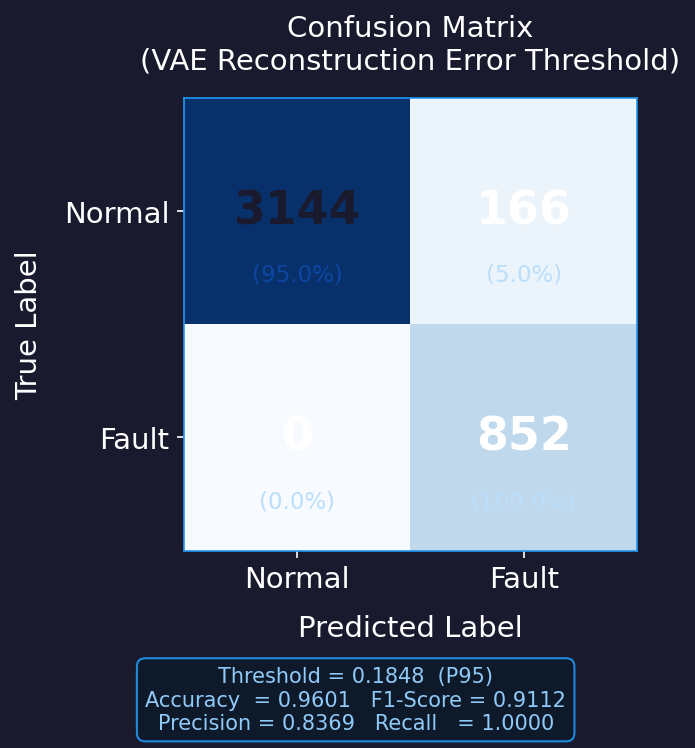
\includegraphics[width=0.80\columnwidth]{confusion_matrix.png}
  \caption{VAE 異常偵測器之混淆矩陣（閾值 $\tau$ 取正常樣本 P95）。
  偽陰性（FN）$= 0$，達到 100\% 故障召回率；
  偽陽性（FP）$= 166$，約佔正常樣本之 5\%（由 P95 閾值設計決定）。}
  \label{fig:cm}
\end{figure}

表~\ref{tab:cm_metrics} 彙整以 P95 閾值對全體樣本進行二元分類之效能指標。
系統在故障召回率（Recall）達到 \textbf{100\%}，即完全無漏報，
符合工業場景「寧可誤報、不可漏報」的設計原則。
5\% 的誤報率（False Alarm Rate）亦為 P95 閾值設計之預期值，
可視實際需求透過調整百分位數靈活控制。

\begin{table}[ht]
\centering
\caption{VAE 二元偵測效能指標（P95 閾值）}
\label{tab:cm_metrics}
\begin{tabular}{lc}
\toprule
\textbf{指標} & \textbf{數值} \\
\midrule
準確率（Accuracy）  & 96.01\% \\
精確率（Precision） & 83.69\% \\
召回率（Recall）    & \textbf{100.00\%} \\
F1-Score            & 91.12\% \\
真陰性（TN）        & 3,144 \\
偽陽性（FP）        & 166 \\
偽陰性（FN）        & \textbf{0} \\
真陽性（TP）        & 852 \\
\bottomrule
\end{tabular}
\end{table}

\subsection{潛在空間視覺化}

\begin{figure}[ht]
  \centering
  \includegraphics[width=0.95\columnwidth]{latent_space.png}
  \caption{32 維潛在均值 $\boldsymbol{\mu}$ 之 t-SNE 投影。
  正常樣本（藍）形成環形流形，與 KL 正則化先驗 $\mathcal{N}(\mathbf{0},\mathbf{I})$ 一致；
  三類故障樣本聚集於中央，位於正常流形之外。}
  \label{fig:latent}
\end{figure}

圖~\ref{fig:latent} 提供系統可信賴性的幾何視覺化證據：
正常資料形成環形流形，KL 散度有效約束其潛在分布；
故障資料在未見過的訓練條件下，自然落在流形之外，
驗證 VAE 的異常偵測機制具備理論一致性。

\subsection{消融實驗}

\begin{figure}[ht]
  \centering
  \includegraphics[width=0.48\columnwidth]{beta_ablation.png}
  \hfill
  \includegraphics[width=0.48\columnwidth]{latent_dim.png}
  \caption{消融實驗。左：KL 權重 $\beta$ 對 AUC-ROC 之影響。
  右：潛在維度對 AUC-ROC 之影響。兩組均維持 AUC$=1.0000$。}
  \label{fig:ablation}
\end{figure}

$\beta\in\{0.1,0.5,1.0,2.0,4.0\}$ 與潛在維度 $\in\{8,16,32,64\}$ 之全部設定
均達 AUC-ROC $=1.0000\pm0.0000$，確認系統對超參數選擇不敏感，具備高度穩健性。
本研究選用 $\beta=1.0$ 以維持標準 VAE 的機率理論一致性，
潛在維度選 32 以提供足夠的表徵容量供未來多機台擴展使用。

% ─────────────────────────────────────────────────────
\section{討論}
% ─────────────────────────────────────────────────────

本研究在 CWRU 資料集上達到完美 AUC，反映該資料集的故障訊號在 12 kHz 採樣下
具備強烈的頻域可分離性。本研究的核心貢獻因此不僅在於效能指標，
更在於提供一套\textbf{可信賴、可解釋、可直接落地}的工業部署管線：

\begin{itemize}
  \item \textbf{無需標注}：訓練資料不含任何故障標籤，適用於新機台上線後立即部署，
        無需等待故障事件累積。
  \item \textbf{可解釋性}：潛在空間的幾何環形結構提供視覺化可解釋依據，
        符合工業 AI 可信賴性（Trustworthy AI）的設計要求。
  \item \textbf{輕量化}：模型大小約 16 MB，訓練僅需一台消費型電腦，
        推論延遲低，具備邊緣裝置部署潛力。
\end{itemize}

\textbf{研究限制：}
CWRU 是實驗室標準資料集，訊號品質高且雜訊少。
未來工作將在更具挑戰性的工業資料集（如 FEMTO-ST、PRONOSTIA）上進行驗證，
並探索模型量化（Quantization）與剪枝（Pruning）以實現即時邊緣推論。

% ─────────────────────────────────────────────────────
\section{結論}
% ─────────────────────────────────────────────────────

本研究設計並實作一套面向工業設備健康監測的可重現無監督異常偵測軟體流程，
以 VAE 軸承振動分析為案例驗證。
流程在模擬工廠真實不平衡分布（79.5\%:20.5\%）的 CWRU 資料集上，
以五折交叉驗證達到 AUC-ROC $= 1.0000\pm0.0000$，
故障重建誤差為正常訊號之 5.2 倍，偵測閾值 $\tau = 0.4778$。
消融實驗確認流程在 KL 權重（0.1--4.0）與潛在維度（8--64）
的廣泛範圍內均具穩健性。

\textbf{研究限制：}本研究目前採用視窗層級隨機切分，
由於相鄰視窗具 50\% 重疊，可能存在資料洩漏問題。
未來工作將改採以原始檔案或負載條件為單位的嚴格切分協議
（file-wise / load-wise split），並在更具挑戰性的資料集（如 FEMTO-ST）上驗證泛化能力。

完整程式碼與實驗結果已公開於：
\url{https://github.com/charmi582/CWRU-VAE}，
供研究者重現與延伸應用。

\section*{誌謝}
感謝凱斯西儲大學軸承資料中心（CWRU Bearing Data Center）
提供公開振動資料集供學術研究使用。

% ─────────────────────────────────────────────────────
\begin{thebibliography}{00}

\bibitem{smith2015rolling}
W.~A. Smith and R.~B. Randall,
``Rolling element bearing diagnostics using the Case Western Reserve
University data: A benchmark study,''
\textit{Mech. Syst. Signal Process.}, vol.~64--65, pp.~100--131, 2015.

\bibitem{kingma2014auto}
D.~P. Kingma and M.~Welling,
``Auto-encoding variational Bayes,''
in \textit{Proc. Int. Conf. Learn. Represent. (ICLR)}, 2014.

\bibitem{zhao2019deep}
R.~Zhao et al.,
``Deep learning and its applications to machine health monitoring,''
\textit{Mech. Syst. Signal Process.}, vol.~115, pp.~213--237, 2019.

\bibitem{an2015variational}
J.~An and S.~Cho,
``Variational autoencoder based anomaly detection using reconstruction
probability,'' \textit{Special Lecture on IE}, vol.~2, no.~1, 2015.

\bibitem{loparo2012}
K.~A. Loparo,
``Bearings vibration data set,'' Case Western Reserve University, 2012.
[Online]. Available: \url{https://engineering.case.edu/bearingdatacenter}

\bibitem{scholkopf2001}
B.~Scholkopf et al.,
``Estimating the support of a high-dimensional distribution,''
\textit{Neural Comput.}, vol.~13, no.~7, pp.~1443--1471, 2001.

\bibitem{breunig2000lof}
M.~M. Breunig et al.,
``LOF: Identifying density-based local outliers,''
in \textit{Proc. ACM SIGMOD}, 2000, pp.~93--104.

\bibitem{liu2008isolation}
F.~T. Liu, K.~M. Ting, and Z.-H. Zhou,
``Isolation forest,'' in \textit{Proc. IEEE ICDM}, 2008, pp.~413--422.

\end{thebibliography}

\end{CJK}
\end{document}
